% -----------------------------------------------------------------------------
% Conteudo AODV-EN. Template base: Prof. Wesley Pacheco Calixto (IFG).
% -----------------------------------------------------------------------------
\chapter{METODOLOGIA}\label{metodologia}

Este capítulo apresenta a metodologia adotada para o desenvolvimento e
avaliação do algoritmo AODV-EN. Inicialmente, realiza-se a
caracterização da pesquisa quanto à sua natureza, abordagem e
procedimentos técnicos. Em seguida, apresenta-se o Design Science
Research (DSR) como paradigma metodológico, justificando sua adequação
ao problema investigado. Na sequência, detalham-se as fases do trabalho
mapeadas às etapas da DSR, o planejamento experimental, as métricas de
avaliação e o algoritmo de referência utilizado para comparação. Por
fim, são descritos os procedimentos de coleta, organização e análise dos
dados experimentais.

\section{Caracterização da
Pesquisa}\label{caracterizauxe7uxe3o-da-pesquisa}

Quanto à sua natureza, esta pesquisa classifica-se como aplicada, pois
visa desenvolver uma solução prática para um problema concreto: a
ausência de suporte nativo a roteamento multi-hop no protocolo ESP-NOW.
Diferentemente da pesquisa básica, que busca ampliar o conhecimento
teórico sem preocupação imediata com aplicação, a pesquisa aplicada
objetiva gerar conhecimento para aplicação prática dirigida à solução de
problemas específicos (GIL, 2017). Quanto aos procedimentos técnicos, a
pesquisa é caracterizada como experimental, uma vez que envolve a
implementação de um protótipo funcional (o algoritmo AODV-EN) e a
realização de testes controlados em ambiente de laboratório. A
experimentação permite manipular variáveis independentes (topologia da
rede, número de nós, padrões de tráfego) e observar seus efeitos sobre
variáveis dependentes (taxa de entrega, latência, consumo energético),
estabelecendo relações de causa e efeito. Quanto à abordagem do
problema, a pesquisa é predominantemente quantitativa, fundamentando-se
na coleta e análise de dados numéricos obtidos através de medições
sistemáticas durante os experimentos. As métricas de desempenho ---
Packet Delivery Ratio (PDR), latência fim-a-fim, Normalized Routing Load
(NRL) e consumo energético --- são quantificadas e submetidas à análise
estatística para validação das hipóteses formuladas.

\section{Design Science Research}\label{design-science-research}

Além da caracterização quanto à natureza, abordagem e procedimentos
técnicos, a pesquisa adota o Design Science Research (DSR) como
paradigma metodológico central para orientar o desenvolvimento e a
avaliação do artefato proposto. A escolha dessa abordagem decorre do
fato de o trabalho não se limitar à análise teórica de um fenômeno, mas
envolver a concepção, implementação e avaliação de uma solução
computacional para um problema prático: a ausência de suporte nativo a
roteamento multi-hop no protocolo ESP-NOW. Nesse contexto, o algoritmo
AODV-EN é compreendido como um artefato computacional, pois materializa
uma proposta de solução por meio de um método de roteamento adaptado às
restrições técnicas do ESP-NOW e implementado em módulos ESP32. Dessa
forma, a DSR fornece uma estrutura adequada para organizar o ciclo de
identificação do problema, definição dos objetivos da solução,
desenvolvimento do artefato, demonstração, avaliação e comunicação dos
resultados.

\subsection{Fundamentos da DSR}\label{fundamentos-da-dsr}

O Design Science Research (DSR) é um paradigma de pesquisa orientado à
criação e avaliação de artefatos inovadores destinados a resolver
problemas práticos. Conforme \citeonline{hevner2004}, enquanto as
ciências naturais buscam descrever e explicar fenômenos existentes, as
ciências do design concentram-se em como as coisas deveriam ser para
atingir determinados objetivos. O propósito do design é, nas palavras de
\citeonline{simon1996}, ``transformar situações existentes em situações
preferidas''. Um artefato, no contexto da DSR, pode assumir diferentes
formas: construtos (vocabulário e símbolos), modelos (abstrações e
representações), métodos (algoritmos e práticas) e instanciações
(implementações funcionais). O algoritmo AODV-EN proposto neste trabalho
constitui simultaneamente um método (especificação do algoritmo de
roteamento) e uma instanciação (implementação funcional em firmware para
ESP32). \citeonline{peffers2007} propuseram um modelo de processo para
condução de pesquisas em DSR composto por seis atividades: (1)
identificação do problema e motivação; (2) definição dos objetivos da
solução; (3) design e desenvolvimento; (4) demonstração; (5) avaliação;
e (6) comunicação. O Quadro 7 apresenta estas etapas e suas descrições.

\textbf{Quadro 7 -- Etapas do Design Science Research segundo
\citeonline{peffers2007}}

{\def\LTcaptype{none} % do not increment counter
\begin{longtable}[]{@{}
  >{\raggedright\arraybackslash}p{(\linewidth - 2\tabcolsep) * \real{0.5000}}
  >{\raggedright\arraybackslash}p{(\linewidth - 2\tabcolsep) * \real{0.5000}}@{}}
\toprule\noalign{}
\begin{minipage}[b]{\linewidth}\raggedright
Etapa DSR
\end{minipage} & \begin{minipage}[b]{\linewidth}\raggedright
Descrição
\end{minipage} \\
\midrule\noalign{}
\endhead
\bottomrule\noalign{}
\endlastfoot
1. Identificação do problema e motivação & Definir o problema de
pesquisa específico e justificar o valor de uma solução. A definição do
problema será utilizada para desenvolver um artefato que possa
efetivamente prover uma solução. \\
2. Definição dos objetivos da solução & Inferir os objetivos de uma
solução a partir da definição do problema e do conhecimento do que é
possível e viável. Os objetivos podem ser quantitativos ou
qualitativos. \\
3. Design e desenvolvimento & Criar o artefato, que pode ser construído,
modelos, métodos ou instâncias. Esta atividade inclui determinar a
funcionalidade desejada do artefato e sua arquitetura. \\
4. Demonstração & Demonstrar a eficácia do artefato na resolução do
problema. Pode envolver experimentação, simulação, estudo de caso, prova
de conceito ou outra atividade apropriada. \\
5. Avaliação & Observar e medir quão bem o artefato suporta uma solução
para o problema. Comparar os objetivos da solução com os resultados
observados na demonstração. \\
6. Comunicação & Comunicar o problema, o artefato, sua utilidade e
novidade, o rigor do design e sua eficácia para pesquisadores e outros
públicos relevantes. \\
\end{longtable}
}

Fonte: Adaptado de \citeonline{peffers2007}.

\subsection{Justificativa da escolha da
DSR}\label{justificativa-da-escolha-da-dsr}

A escolha metodológica para este trabalho justifica-se por sua aderência
ao tipo de problema investigado e à natureza da contribuição pretendida.
Como a pesquisa envolve a concepção, implementação e avaliação de um
artefato computacional, a DSR é adequada para estruturar o ciclo de
desenvolvimento e validação da solução proposta. a) \textbf{Natureza do
problema}: o problema investigado, relacionado à ausência de roteamento
multi-hop nativo no protocolo ESP-NOW, possui natureza técnica e
prática, demandando uma solução concreta na forma de um artefato
funcional, e não apenas a compreensão teórica do fenômeno; b)
\textbf{Tipo de contribuição:} a contribuição principal do trabalho é
prescritiva, pois busca indicar como construir uma solução para o
problema identificado, e não apenas descritiva, isto é, limitada à
explicação de como determinado fenômeno ocorre. Essa característica
alinha-se à epistemologia das ciências do design; c) \textbf{Ciclo
construir-avaliar}: a DSR estrutura formalmente o ciclo iterativo de
construção e avaliação de artefatos, fornecendo um arcabouço
metodológico rigoroso para orientar o processo de desenvolvimento e
validação do algoritmo proposto; d) \textbf{Adequação a algoritmos}:
conforme \citeonline{marchsmith1995}, algoritmos constituem um tipo
clássico de artefato em pesquisas orientadas pelo Design Science
Research, sendo essa metodologia amplamente utilizada em trabalhos que
envolvem o desenvolvimento de novos métodos computacionais; e)
\textbf{Rigor e relevância}: a DSR equilibra o rigor científico, por
meio da fundamentação teórica e da avaliação sistemática, com a
relevância prática, voltada à solução de um problema real, atendendo aos
critérios de qualidade esperados em pesquisas na área de Engenharia de
Software.

\section{Mapeamento das Fases do Trabalho às Etapas da
DSR}\label{mapeamento-das-fases-do-trabalho-uxe0s-etapas-da-dsr}

O presente trabalho está organizado em cinco fases, que foram mapeadas
às etapas do modelo de processo DSR de \citeonline{peffers2007}. O
Quadro 8 apresenta este mapeamento, relacionando cada fase do trabalho à
respectiva etapa DSR, suas atividades específicas e produtos esperados.

\textbf{Quadro 8 -- Mapeamento das fases do trabalho às etapas da DSR}

{\def\LTcaptype{none} % do not increment counter
\begin{longtable}[]{@{}
  >{\raggedright\arraybackslash}p{(\linewidth - 6\tabcolsep) * \real{0.2500}}
  >{\raggedright\arraybackslash}p{(\linewidth - 6\tabcolsep) * \real{0.2500}}
  >{\raggedright\arraybackslash}p{(\linewidth - 6\tabcolsep) * \real{0.2500}}
  >{\raggedright\arraybackslash}p{(\linewidth - 6\tabcolsep) * \real{0.2500}}@{}}
\toprule\noalign{}
\begin{minipage}[b]{\linewidth}\raggedright
Fase
\end{minipage} & \begin{minipage}[b]{\linewidth}\raggedright
Etapa DSR
\end{minipage} & \begin{minipage}[b]{\linewidth}\raggedright
Atividades
\end{minipage} & \begin{minipage}[b]{\linewidth}\raggedright
Produtos
\end{minipage} \\
\midrule\noalign{}
\endhead
\bottomrule\noalign{}
\endlastfoot
Fase 1: Revisão Bibliográfica & 1. Identificação do problema e motivação
& • Levantamento da literatura sobre AODV, ESP-NOW e redes mesh •
Identificação das limitações do ESP-NOW • Análise de soluções existentes
e lacunas & • Referencial teórico • Trabalhos correlatos • Definição do
problema \\
Fase 2: Projeto do Algoritmo AODV-EN & 2. Definição dos objetivos / 3.
Design e desenvolvimento & • Especificação dos requisitos funcionais •
Definição da arquitetura do algoritmo • Projeto das adaptações do AODV
para ESP-NOW • Definição das estruturas de dados e mensagens & •
Diagramas de arquitetura • Pseudocódigo \\
Fase 3: Implementação e Ambiente de Testes & 3. Design e desenvolvimento
& • Codificação do firmware para ESP32 • Implementação do algoritmo
baseline (Flooding) • Montagem do ambiente físico de testes •
Desenvolvimento de ferramentas de coleta & • Código-fonte do Flooding •
Testbed operacional \\
Fase 4: Execução dos Experimentos & 4. Demonstração & • Execução dos
cenários experimentais • Coleta de métricas (PDR, latência, NRL,
energia) • Registro de logs e eventos & • Datasets de medições • Logs de
execução \\
Fase 5: Análise e Discussão & 5. Avaliação e 6. Comunicação & • Análise
estatística dos resultados • Comparação AODV-EN vs.~Flooding
vs.~literatura • Verificação das hipóteses • Elaboração do TCC & •
Análise de resultados • Conclusões • Documento final \\
\end{longtable}
}

Fonte: Elaborado pelos autores.

A Figura 1 apresenta, de forma sintética, o fluxo metodológico adotado
nesta pesquisa, evidenciando a relação entre o problema investigado, a
abordagem Design Science Research, as fases do trabalho e a etapa de
avaliação experimental. A representação contribui para visualizar a
sequência lógica das atividades desenvolvidas ao longo da pesquisa.

\begin{figure}
\centering
\pandocbounded{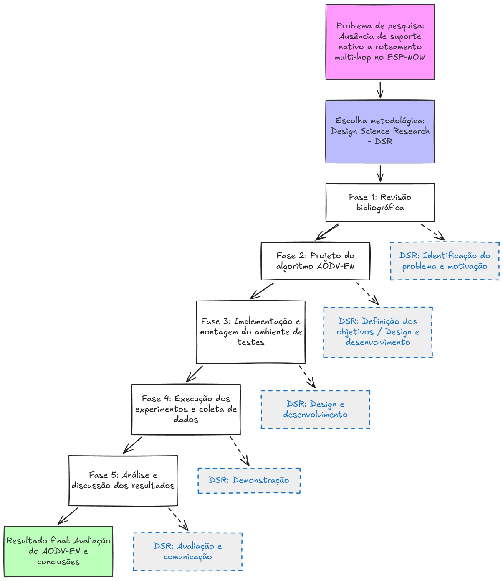
\includegraphics[keepaspectratio,alt={Figura 1 -- Fluxo metodológico da pesquisa}]{figuras/image1.png}}
\caption{Figura 1 -- Fluxo metodológico da pesquisa}
\end{figure}

\subsection{Fase 1: Revisão
Bibliográfica}\label{fase-1-revisuxe3o-bibliogruxe1fica}

A primeira fase corresponde à etapa de Identificação do Problema e
Motivação da DSR. Nesta fase, foi realizado o levantamento bibliográfico
para fundamentar teoricamente o trabalho e identificar com precisão as
lacunas existentes na literatura. O levantamento bibliográfico
concentrou-se em três eixos temáticos: (i) o protocolo AODV e suas
variantes, tendo como referência primária a RFC 3561; (ii) o protocolo
ESP-NOW, suas características técnicas e limitações; e (iii) soluções
existentes para redes mesh em plataformas embarcadas de baixo custo. As
fontes consultadas incluíram bases de dados científicas (IEEE Xplore,
ACM Digital Library, ScienceDirect), documentação técnica oficial
(Espressif Systems, IETF RFCs) e repositórios de projetos open-source
(GitHub). Os critérios de seleção priorizaram publicações recentes
(2021-2025) que abordassem especificamente ESP-NOW ou roteamento em
redes de sensores de baixo custo.

\subsection{Fase 2: Projeto do Algoritmo
AODV-EN}\label{fase-2-projeto-do-algoritmo-aodv-en}

A segunda fase corresponde às etapas de Definição dos Objetivos da
Solução e início do Design e Desenvolvimento. Nesta fase, são
especificados os requisitos funcionais e não-funcionais do artefato,
definida sua arquitetura e projetadas as adaptações necessárias do
protocolo AODV original para operação sobre ESP-NOW. O projeto do
AODV-EN parte dos princípios do protocolo AODV, especialmente quanto à
descoberta de rotas sob demanda, ao uso de mensagens de controle, à
manutenção de tabelas de roteamento e ao tratamento de falhas de enlace.
A partir desses princípios, foram definidas adaptações necessárias para
sua operação sobre ESP-NOW. As principais decisões de projeto incluem:
a) \textbf{Gerenciamento de peers}: política LRU (Least Recently Used)
para gerenciamento dinâmico da tabela de peers, permitindo comunicação
com mais de 20 nós ao longo do tempo dentro do limite simultâneo imposto
pelo ESP-NOW; b) \textbf{Disseminação de mensagens RREQ}:
\emph{flooding} controlado sobre \emph{broadcast} de enlace do ESP-NOW
(FF:FF:FF:FF:FF:FF), com supressão de duplicatas por cache de
identificadores e limite de propagação por TTL, preservando a semântica
de difusão do AODV original; c) \textbf{Métrica de roteamento}: métrica
híbrida combinando contagem de saltos (hop count) e qualidade de enlace
(RSSI), permitindo seleção de rotas que otimizem simultaneamente
distância lógica e confiabilidade esperada; d) \textbf{Estruturas de
dados}: tabela de roteamento, tabela de peers com timestamps, buffer de
RREQ IDs para detecção de duplicatas, e lista de precursores para
notificação de falhas.

\subsection{Fase 3: Implementação e Montagem do Ambiente de
Testes}\label{fase-3-implementauxe7uxe3o-e-montagem-do-ambiente-de-testes}

A terceira fase dá continuidade à etapa de Design e Desenvolvimento,
materializando o projeto em código funcional e preparando o ambiente
para os experimentos. A implementação será realizada em linguagem C
utilizando o framework ESP-IDF (Espressif IoT Development Framework). O
código será organizado em módulos: gerenciamento de peers, descoberta de
rotas, manutenção de rotas, encaminhamento de pacotes e interface de
coleta de métricas. Paralelamente, será implementado o algoritmo
Flooding para fins de comparação. O ambiente de testes (testbed) será
composto por 10 módulos ESP32 DevKit V1, alimentados por fontes USB 5V.
A disposição física dos nós seguirá as topologias definidas na Seção
4.4. Cada nó executará o mesmo firmware, sendo configurado com
identificador único através de variáveis de compilação.

\subsection{Fase 4: Execução dos Experimentos e Coleta de
Dados}\label{fase-4-execuuxe7uxe3o-dos-experimentos-e-coleta-de-dados}

A quarta fase corresponde à etapa de Demonstração da DSR, onde o
artefato é exercitado em cenários representativos para demonstrar sua
eficácia na resolução do problema. Os experimentos seguirão o
planejamento detalhado na Seção 4.4. Para cada cenário experimental,
serão realizadas múltiplas execuções (mínimo de 30 repetições) para
garantir significância estatística. As métricas serão coletadas
automaticamente pelo firmware e transmitidas para um nó coordenador, que
as registra em arquivos de log para posterior análise.

\subsection{Fase 5: Análise e Discussão dos
Resultados}\label{fase-5-anuxe1lise-e-discussuxe3o-dos-resultados}

A quinta fase corresponde às etapas de Avaliação e Comunicação da DSR.
Os dados coletados serão submetidos a análise estatística utilizando
técnicas descritivas (média, desvio padrão, intervalos de confiança) e
inferenciais (testes de hipóteses) quando apropriado. A avaliação
comparará os resultados do AODV-EN com: (i) o algoritmo Flooding
implementado localmente; e (ii) resultados reportados na literatura para
soluções similares, como o BRAM-NOW de Cujilema et al.~(2023). A
comunicação dos resultados será realizada através deste TCC e,
potencialmente, através de publicação em evento científico.

\section{Planejamento Experimental}\label{planejamento-experimental}

O planejamento experimental foi definido com o objetivo de avaliar o
comportamento do algoritmo AODV-EN em diferentes condições de operação
de uma rede mesh baseada em ESP-NOW. Considerando que a proposta envolve
roteamento multi-hop, seleção de rotas, manutenção da comunicação e
recuperação diante de falhas, os experimentos foram organizados em
cenários capazes de representar situações progressivamente mais
complexas de comunicação multi-hop. A avaliação será realizada por meio
da comparação entre o AODV-EN e um algoritmo de referência baseado em
Flooding, permitindo observar diferenças quanto à confiabilidade da
entrega, latência fim-a-fim, carga de controle e consumo energético
estimado.

\subsection{Cenários experimentais}\label{cenuxe1rios-experimentais}

Os experimentos serão conduzidos em quatro cenários distintos,
projetados para avaliar aspectos complementares do desempenho do
algoritmo proposto. O cenário C1 avalia o comportamento multi-hop básico
em uma topologia linear; o cenário C2 verifica o encaminhamento em uma
estrutura hierárquica; o cenário C3 analisa a seleção de rotas em uma
malha parcial com caminhos alternativos; e o cenário C4 observa a
capacidade de detecção de falhas e recuperação da comunicação.

\textbf{Quadro 9 -- Configuração dos cenários experimentais}

{\def\LTcaptype{none} % do not increment counter
\begin{longtable}[]{@{}
  >{\raggedright\arraybackslash}p{(\linewidth - 6\tabcolsep) * \real{0.2500}}
  >{\raggedright\arraybackslash}p{(\linewidth - 6\tabcolsep) * \real{0.2500}}
  >{\raggedright\arraybackslash}p{(\linewidth - 6\tabcolsep) * \real{0.2500}}
  >{\raggedright\arraybackslash}p{(\linewidth - 6\tabcolsep) * \real{0.2500}}@{}}
\toprule\noalign{}
\begin{minipage}[b]{\linewidth}\raggedright
Cenário
\end{minipage} & \begin{minipage}[b]{\linewidth}\raggedright
Topologia
\end{minipage} & \begin{minipage}[b]{\linewidth}\raggedright
Configuração
\end{minipage} & \begin{minipage}[b]{\linewidth}\raggedright
Objetivo
\end{minipage} \\
\midrule\noalign{}
\endhead
\bottomrule\noalign{}
\endlastfoot
C1: Linear & Cadeia & • 5 nós em linha (N1→N2→N3→N4→N5) • Distância
entre nós: 10m • Comunicação: N1↔N5 • 4 saltos obrigatórios & Avaliar
comportamento multi-hop básico e latência acumulada por salto \\
C2: Árvore & Hierárquica & • 7 nós em estrutura de árvore • 1 raiz, 2
nós nível 1, 4 folhas • Comunicação: folhas↔raiz • Máximo 2 saltos &
Avaliar encaminhamento hierárquico e agregação de tráfego \\
C3: Mesh Parcial & Redundante & • 6 nós com múltiplos caminhos • Cada nó
alcança 2-3 vizinhos • Comunicação: extremidades • Rotas alternativas
disponíveis & Avaliar seleção de rotas e capacidade de utilizar caminhos
alternativos \\
C4: Falha & Linear com interrupção & • Cenário C1 com falha induzida •
Nó N3 desligado após 60s • Observação da recuperação & Avaliar detecção
de falha e capacidade de auto-recuperação (self-healing) \\
\end{longtable}
}

Fonte: Elaborado pelos autores.

\subsection{Parâmetros dos
experimentos}\label{paruxe2metros-dos-experimentos}

Os parâmetros experimentais foram definidos com o objetivo de manter
condições equivalentes de comparação entre o AODV-EN e o algoritmo de
referência. Assim, variáveis como número de nós, tamanho do payload,
taxa de envio, duração das execuções e número de repetições foram
padronizadas para ambos os algoritmos, variando apenas os parâmetros
específicos de cada abordagem. No caso do AODV-EN, são considerados
parâmetros próprios do protocolo, como o intervalo de mensagens HELLO e
o tempo de validade das rotas ativas. Para o Flooding, define-se o valor
máximo de TTL, utilizado para limitar a propagação dos pacotes e evitar
retransmissões indefinidas.

\textbf{Quadro 10 -- Parâmetros dos experimentos}

{\def\LTcaptype{none} % do not increment counter
\begin{longtable}[]{@{}
  >{\centering\arraybackslash}p{(\linewidth - 4\tabcolsep) * \real{0.3333}}
  >{\centering\arraybackslash}p{(\linewidth - 4\tabcolsep) * \real{0.3333}}
  >{\centering\arraybackslash}p{(\linewidth - 4\tabcolsep) * \real{0.3333}}@{}}
\toprule\noalign{}
\begin{minipage}[b]{\linewidth}\centering
Parâmetro
\end{minipage} & \begin{minipage}[b]{\linewidth}\centering
AODV-EN
\end{minipage} & \begin{minipage}[b]{\linewidth}\centering
Flooding
\end{minipage} \\
\midrule\noalign{}
\endhead
\bottomrule\noalign{}
\endlastfoot
Número de nós & 5-10 (conforme cenário) & 5-10 (conforme cenário) \\
Tamanho do payload & 32 bytes & 32 bytes \\
Taxa de envio (steady state) & 1 pacote/segundo & 1 pacote/segundo \\
Duração de cada execução & 300 segundos (5 min) & 300 segundos (5
min) \\
Repetições por cenário & 30 & 30 \\
HELLO\_INTERVAL & 2.000 ms & N/A \\
ACTIVE\_ROUTE\_TIMEOUT & 10.000 ms & N/A \\
TTL máximo (Flooding) & N/A & 5 saltos \\
\end{longtable}
}

\section{}\label{section}

\section{}\label{section-1}

\section{}\label{section-2}

\section{}\label{section-3}

\section{}\label{section-4}

\section{}\label{section-5}

Fonte: Elaborado pelos autores.

\section{Métricas de Avaliação}\label{muxe9tricas-de-avaliauxe7uxe3o}

A avaliação do desempenho do algoritmo AODV-EN será realizada por meio
de quatro métricas complementares: Packet Delivery Ratio (PDR), latência
fim-a-fim, Normalized Routing Load (NRL) e consumo energético estimado.
Essas métricas foram selecionadas por sua recorrência na literatura de
redes ad-hoc e por sua adequação ao contexto de redes de sensores sem
fio com recursos limitados. O PDR permite avaliar a confiabilidade da
comunicação; a latência fim-a-fim indica o desempenho temporal da
entrega dos pacotes; o NRL mede o overhead de controle introduzido pelo
protocolo; e o consumo energético estimado permite analisar o impacto
das transmissões sobre a autonomia dos dispositivos.

\textbf{Quadro 11 -- Métricas de avaliação de desempenho}

{\def\LTcaptype{none} % do not increment counter
\begin{longtable}[]{@{}
  >{\raggedright\arraybackslash}p{(\linewidth - 4\tabcolsep) * \real{0.3333}}
  >{\raggedright\arraybackslash}p{(\linewidth - 4\tabcolsep) * \real{0.3333}}
  >{\raggedright\arraybackslash}p{(\linewidth - 4\tabcolsep) * \real{0.3333}}@{}}
\toprule\noalign{}
\begin{minipage}[b]{\linewidth}\raggedright
Métrica
\end{minipage} & \begin{minipage}[b]{\linewidth}\raggedright
Definição
\end{minipage} & \begin{minipage}[b]{\linewidth}\raggedright
Fórmula
\end{minipage} \\
\midrule\noalign{}
\endhead
\bottomrule\noalign{}
\endlastfoot
PDR (Packet Delivery Ratio) & Razão entre pacotes de dados recebidos no
destino e pacotes enviados pela origem. Indica a confiabilidade da
comunicação. & PDR = (Pacotes recebidos / Pacotes enviados) × 100\% \\
Latência Fim-a-Fim & Tempo decorrido entre o envio de um pacote pela
origem e sua recepção no destino. Inclui tempo de processamento,
enfileiramento e transmissão em cada salto. & L = t\_recepção -
t\_envio \\
NRL (Normalized Routing Load) & Razão entre o número de pacotes de
controle transmitidos e o número de pacotes de dados entregues. Indica a
eficiência do protocolo em termos de overhead. & NRL = Pacotes de
controle / Pacotes de dados entregues \\
Consumo Energético Estimado & Estimativa do consumo de energia baseada
no número de transmissões e no perfil de consumo do ESP32. Permite
projetar autonomia com bateria. & E = Σ(N\_tx × E\_tx + N\_rx × E\_rx +
t\_idle × P\_idle) \\
\end{longtable}
}

Fonte: Elaborado pelos autores.

Para cada métrica, serão calculados: média aritmética, desvio padrão e
intervalo de confiança de 95\%. Os resultados serão apresentados em
tabelas e gráficos comparativos entre AODV-EN e Flooding.

\section{Algoritmo de Referência para Comparação:
Flooding}\label{algoritmo-de-referuxeancia-para-comparauxe7uxe3o-flooding}

Para estabelecer uma base de comparação experimental, será implementado
um algoritmo de referência baseado em Flooding sobre ESP-NOW. O Flooding
é a abordagem mais básica para disseminação de mensagens em redes sem
infraestrutura, consistindo na retransmissão de cada pacote recebido
para todos os vizinhos, exceto aquele de quem o pacote foi recebido.

\subsection{Especificação do algoritmo
Flooding}\label{especificauxe7uxe3o-do-algoritmo-flooding}

O algoritmo de referência baseado em Flooding será implementado com as
seguintes características: a) \textbf{Estrutura do pacote}: cada pacote
contém identificador único (origem + número de sequência), endereço de
origem, endereço de destino, TTL (Time-To-Live) e payload de dados; b)
\textbf{Detecção de duplicatas}: cada nó mantém um buffer circular com
os últimos N identificadores de pacotes recebidos (N=100). Pacotes com
identificadores já presentes no buffer são descartados; c)
\textbf{Controle de TTL}: o TTL é decrementado a cada salto. Pacotes com
TTL=0 não são retransmitidos, limitando o alcance do flooding e
prevenindo loops infinitos; d) \textbf{Retransmissão}: ao receber um
pacote não-duplicado com TTL\textgreater0 e destino diferente do próprio
nó, o pacote é retransmitido em um único \emph{broadcast} de enlace
ESP-NOW (FF:FF:FF:FF:FF:FF), conforme a definição clássica de
\emph{flooding} --- uma retransmissão por nó, suprimida por duplicatas e
limitada por TTL; e) \textbf{Entrega ao destino}: quando o pacote
alcança o nó de destino, o payload é entregue à aplicação e a recepção é
registrada para cálculo das métricas.

\subsection{Justificativa da escolha do Flooding como algoritmo de
referência}\label{justificativa-da-escolha-do-flooding-como-algoritmo-de-referuxeancia}

A escolha do Flooding como algoritmo de comparação justifica-se por: a)
\textbf{Simplicidade}: é o algoritmo mais simples possível para
comunicação multi-hop, servindo como limite inferior de complexidade de
implementação; b) \textbf{Garantia de entrega}: em redes conectadas, o
Flooding garante que o pacote alcançará o destino (se existir caminho),
servindo como referência de PDR máximo alcançável; c) \textbf{Overhead
elevado}: o Flooding representa o extremo oposto em termos de
eficiência, permitindo quantificar os ganhos obtidos pelo roteamento
inteligente do AODV-EN; d) \textbf{Ausência de estado}: não requer
tabelas de roteamento ou manutenção de rotas, isolando o impacto desses
mecanismos no AODV-EN. A comparação entre o AODV-EN e o Flooding
permitirá avaliar a relação entre complexidade de implementação e
eficiência de comunicação. Embora o AODV-EN apresente maior complexidade
por envolver descoberta e manutenção de rotas, espera-se que ele
proporcione menor carga de controle, menor consumo energético estimado e
desempenho comparável em termos de taxa de entrega de pacotes.

\section{Coleta e Análise dos
Dados}\label{coleta-e-anuxe1lise-dos-dados}

Os dados experimentais serão coletados a partir dos registros gerados
durante a execução dos cenários de teste. Esses registros incluirão
informações sobre pacotes enviados, pacotes recebidos, mensagens de
controle, eventos de retransmissão, falhas de comunicação, atualizações
de rota e tempos de envio e recepção.
\begin{figure}[H]
\centering
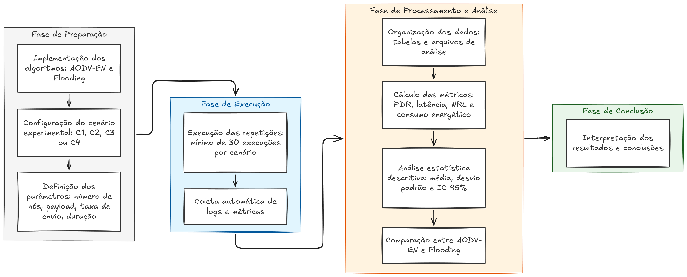
\includegraphics[width=0.85\textwidth,keepaspectratio]{figuras/image2.png}
\caption{Figura 2 -- Fluxo de execução dos experimentos e análise dos dados}
\end{figure}
A Figura 2 sintetiza o fluxo de execução dos experimentos e de
tratamento dos dados, desde a configuração do ambiente experimental até
a comparação dos resultados obtidos para o AODV-EN e o algoritmo de
referência baseado em Flooding. Para garantir a rastreabilidade dos
experimentos, cada execução deverá ser identificada pelo cenário
avaliado, algoritmo utilizado, número da repetição, configuração dos nós
e arquivos de log correspondentes. Essa organização permitirá relacionar
os resultados obtidos às condições específicas de cada execução
experimental. Após a coleta, os dados serão organizados em tabelas e
submetidos à análise estatística descritiva, considerando média, desvio
padrão e intervalo de confiança de 95\% para cada métrica avaliada. A
análise será realizada por cenário e por algoritmo, possibilitando a
comparação direta entre os resultados do AODV-EN e do algoritmo de
referência baseado em Flooding. Execuções com falhas de instrumentação,
perda de registros, reinicialização inesperada dos dispositivos ou
divergência de configuração serão desconsideradas e repetidas, a fim de
preservar a consistência dos dados analisados. A partir dos resultados
consolidados, será avaliado se o AODV-EN, apresenta ganhos em eficiência
de comunicação, mantendo desempenho compatível em termos de
confiabilidade e latência.
